\chapter{Experiment}
\section{Slab Waveguide}



\section{Quadratic single-mode strip waveguide}
The next step was to simulate a three dimensional strip waveguide in air with a higth and a lenght of 0.356~$upmu$m and a core refractive index $n$~=~3.03 in air.
The lenght of the waveguide was 100~$\upmu$m.

Figure \ref{fig:2_index} shows the index profile of the waveguide.

\begin{figure}%
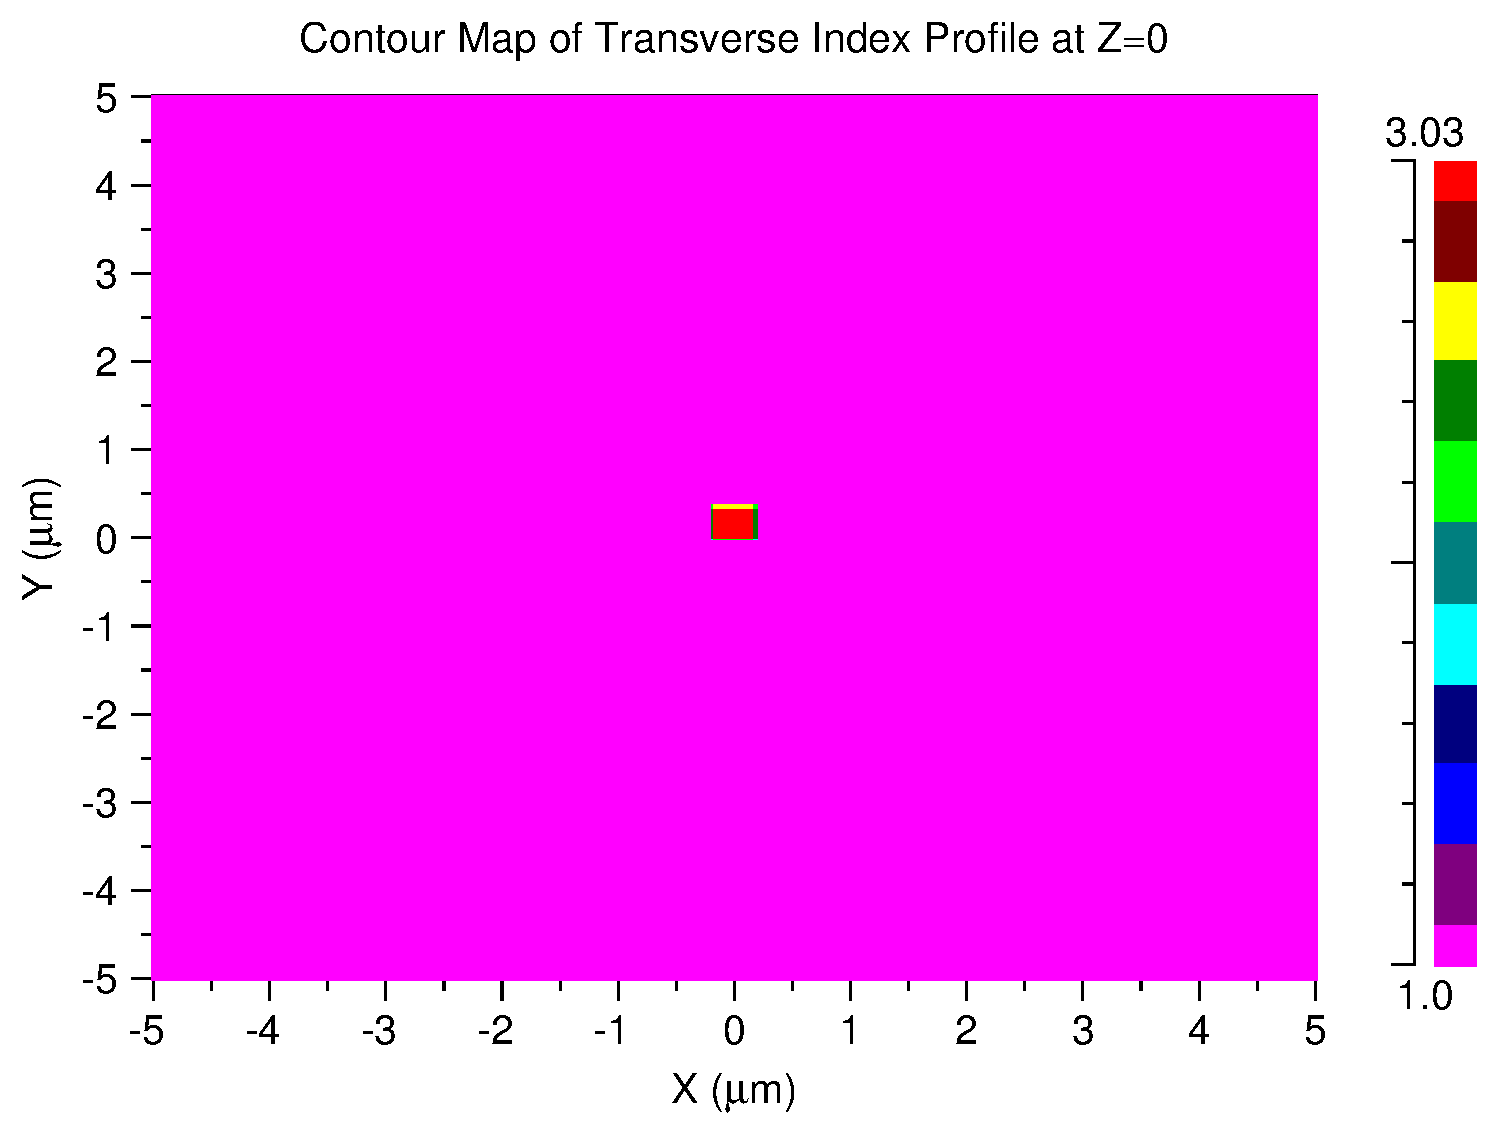
\includegraphics[width=.5\columnwidth]{Grafiken/2_index}%
\caption{index profile of the quadratic single-mode strip waveguide.}%
\label{fig:2_index}%
\end{figure}

The excitation of the field is Gaussian and and has an offset in x direction by 0.25 times the width and in y direction by 0.25 times the hight of the waveguide.
For this waveguide all modes wer calculated at a frequency of 200~THz by using the correlation method and a grid size in x/y/z-direction of 0.02/0.02/0.05. 



\begin{figure}%
\centering
%\begin{adjustwidth}{0cm}{0cm}
	\subfloat[  ]{\includegraphics[totalheight=6 cm]{Grafiken/  }\label{fig:}}
	\subfloat[  ]{\includegraphics[totalheight=4 cm]{Grafiken/  } \label{fig:  }}\\%
	\subfloat[  ]{\includegraphics[totalheight=4 cm]{Grafiken/  }\label{fig:  }}
	\subfloat[  ]{\includegraphics[totalheight=4 cm]{Grafiken/  } \label{fig:  }}
%\end{adjustwidth}
\caption{}%
\label{fig:2_modes}%
\end{figure}




\section{Design of a SOI strip waveguide}